\chapter{Arhitektura i dizajn sustava}
		
		\textbf{\textit{dio 1. revizije}}\\

		\textit{ Potrebno je opisati stil arhitekture te identificirati: podsustave, preslikavanje na radnu platformu, spremišta podataka, mrežne protokole, globalni upravljački tok i sklopovsko-programske zahtjeve. Po točkama razraditi i popratiti odgovarajućim skicama:}
	\begin{itemize}
		\item 	\textit{izbor arhitekture temeljem principa oblikovanja pokazanih na predavanjima (objasniti zašto ste baš odabrali takvu arhitekturu)}
		\item 	\textit{organizaciju sustava s najviše razine apstrakcije (npr. klijent-poslužitelj, baza podataka, datotečni sustav, grafičko sučelje)}
		\item 	\textit{organizaciju aplikacije (npr. slojevi frontend i backend, MVC arhitektura) }		
	\end{itemize}

	
		

		

				
		\section{Baza podataka}
			
			
		\textit{Kao sustav za upravljanje bazama podataka za našu aplikaciju odabrali smo PostgreSQL. To je otvoren sustav za upravljanje bazama koji omogućuje pohranu, upravljanje i analizu podataka. }
			
		\textit{Sama baza podataka sadržavat će šest tablica. One će služiti za pohranu podataka o korisnicima te njihovom korištenju aplikacije. Korištenje će se spremati u obliku događaja koje stvaraju ili posjećuju te recenzija koje pišu za određene događaje. Isto tako spremat će se sama zainteresiranost za događaje te notifikacije koje posjetitelji žele primati za događaje s određenim karakteristikama.}
			
		\textit{Sami odabir PostgreSQL-a je u njegovoj pouzdanosti, skalabilnosti i podrške za napredne SQL funkcionalnosti, što će nam omogućiti lakše te učinkovitije upravljanje podacima.
			Baza podataka ove aplikacije sastoji se od sljedećih entiteta: }
			\begin{itemize}
			\item 	\textit{Korisnik}		
			\item 	\textit{Organizator}	
			\item 	\textit{Događaj}
			\item 	\textit{Recenzija}
			\item 	\textit{Zainteresiranost}
			\item 	\textit{Notifikacija}
		\end{itemize}
		
		
			\subsection{Opis tablica}
			

				\textit{\textbf{Korisnik} -  ovaj entitet sadržava sve važne informacije o korisniku aplikacije. Sadrži atribute: korisnik\_id koji je automatski dodijeljen, username, lozinka, email i uloga u aplikaciji. Ovaj entitet u vezi je Many-to-One s entitetom organizator preko atributa organizator\_id.}
				
				
				\begin{longtblr}[
					label=none,
					entry=none
					]{
						width = \textwidth,
						colspec={|X[7,l]|X[6, l]|X[20, l]|}, 
						rowhead = 1,
					} %definicija širine tablice, širine stupaca, poravnanje i broja redaka naslova tablice
					\hline \SetCell[c=3]{c}{\textbf{korisnik}}	 \\ \hline[3pt]
					\SetCell{LightGreen}korisnik\_id & INT	&  	Primarni ključ tablice, dodjeljuje se automatski  	\\ \hline
					username	& VARCHAR & Jedinstveno ime koje korisnik odabire tijekom registracije  	\\ \hline 
					lozinka & VARCHAR & Lozinka koju korisnik odabire tijekom registracije  \\ \hline 
					email & VARCHAR	&  Jedinstveni email korisnika		\\ \hline 
					uloga & SMALL INT/INT &  Uloga koju korisnik ima unutar aplikacije(admin, posjetitelj, organizator)		\\ \hline 
				\end{longtblr}
				
							\textit{\textbf{Organizator } -  Ovaj entitet sadržava informacije o organizatoru događaja. Sadrži atribute: organizator\_id, naziv\_organizacije, adresa, poveznica, clanarina. Ovaj entitet u vezi je One-to-Many s entitetom dogadaj preko atributa organizator\_id.}
			
			
			\begin{longtblr}[
				label=none,
				entry=none
				]{
					width = \textwidth,
					colspec={|X[9,l]|X[6, l]|X[20, l]|}, 
					rowhead = 1,
				} %definicija širine tablice, širine stupaca, poravnanje i broja redaka naslova tablice
				\hline \SetCell[c=3]{c}{\textbf{organizator}}	 \\ \hline[3pt]
				\SetCell{LightGreen}organizator\_id & INT	&  	Primarni ključ tablice, ujedno i strani ključ iz tablice korisnik 	\\ \hline
				naziv\_organizacije	& VARCHAR & Naziv organizacije kojoj pripada organizator  	\\ \hline 
				adresa & VARCHAR & Adresa organizacije  \\ \hline 
				poveznica & VARCHAR	&  Poveznica na web stranicu organizacije		\\ \hline 
				clanarina & BOOLEAN &  Plaćena članarina		\\ \hline 
			\end{longtblr}
			
							\textit{\textbf{Dogadaj } -  ovaj entitet sadržava informacije o događaju. Sadrži atribute: dogadaj\_id, organizator\_id, naziv\_dogadaja, vrsta, lokacija, trajanje, vrijeme\_pocetka, cijena\_ulaznice, opis, galerija. Ovaj entitet u vezi je Many-to-One s entitetom Organizator preko atributa organizator\_id te u vezi One-to-Many s entitetom recenzija preko atributa dogadaj\_id.}
			
			
			\begin{longtblr}[
				label=none,
				entry=none
				]{
					width = \textwidth,
					colspec={|X[7,l]|X[6, l]|X[20, l]|}, 
					rowhead = 1,
				} %definicija širine tablice, širine stupaca, poravnanje i broja redaka naslova tablice
				\hline \SetCell[c=3]{c}{\textbf{dogadaj}}	 \\ \hline[3pt]
				\SetCell{LightGreen}dogadaj\_id & INT	&  	Primarni ključ tablice, dodjeljuje se automatski  	\\ \hline				\SetCell{LightBlue} organizator\_id	& INT & Strani ključ iz tablice organizator koji se odnosi na njegov ID  	\\ \hline 
				naziv\_dogadaja	& VARCHAR & Naziv događaja  	\\ \hline 
				vrsta & VARCHAR & Vrsta događaja(koncert, kazališna predstava ...)  \\ \hline 
				lokacija & VARCHAR	&  Lokacija događaja		\\ \hline 
				opis\_lokacije & VARCHAR & Kratki opis lokacije, adresa, kat …	\\ \hline 
				trajanje & INTERVAL & Trajanje događaja u danima \\ \hline 
				vrijeme\_pocetka & TIMESTAMP & Datum i vrijeme početka događaja \\ \hline 
				cijena\_ulaznice & NUMERIC & Cijena ulaznice na događaj \\ \hline 
				opis & VARCHAR & Kratki opis samog događaja \\ \hline 
				galerija & VARCHAR & Link do web stranice gdje se nalaze video snimke ili fotografije \\ \hline  
			\end{longtblr}
			
							\textit{\textbf{Recenzija} -  ovaj entitet sadržava informacije o recenziji događaja. Sadrži atribute: recenzija\_id, posjetitelj\_id, događaj\_id, tekst, ocjena. Ovaj entitet u vezi je Many-to-One s entitetom korisnik preko atributa posjetitelj\_id te u vezi Many-to-One s entitetom dogadaj preko atributa dogadaj\_id.}
			
			
			\begin{longtblr}[
				label=none,
				entry=none
				]{
					width = \textwidth,
					colspec={|X[7,l]|X[6, l]|X[20, l]|}, 
					rowhead = 1,
				} %definicija širine tablice, širine stupaca, poravnanje i broja redaka naslova tablice
				\hline \SetCell[c=3]{c}{\textbf{recenzija}}	 \\ \hline[3pt]
				\SetCell{LightGreen}recenzija\_id & INT	&  	Primarni ključ tablice, dodjeljuje se automatski  	\\ \hline
				\SetCell{LightBlue}posjetitelj\_id	& INT & Strani ključ iz tablice korisnik koji se odnosi na njegov ID	\\ \hline 
				\SetCell{LightBlue}dogadaj\_id & INT & Strani ključ iz tablice dogadaj koji se odnosi na njegov ID \\ \hline 
				tekst & VARCHAR	&  Kratki tekst recenzije	\\ \hline 
				ocjena & SMALL INT/INT & Ocjena od 1-10, opcionalna	\\ \hline 
			\end{longtblr}
			
							\textit{\textbf{Zainteresiranost} -  ovaj entitet sadržava informacije o zainteresiranosti posjetitelja za određeni događaj. Sadrži atribute: zainteresiranost\_id, posjetitelj\_id, dogadaj\_id, kategorija, obavijesti. Ovaj entitet u vezi je Many-to-One s entitetom korisnik preko atributa posjetitelj\_id te u vezi Many-to-One s entitetom dogadaj preko atributa dogadaj\_id.}
			
			
			\begin{longtblr}[
				label=none,
				entry=none
				]{
					width = \textwidth,
					colspec={|X[9,l]|X[6, l]|X[20, l]|}, 
					rowhead = 1,
				} %definicija širine tablice, širine stupaca, poravnanje i broja redaka naslova tablice
								\hline \SetCell[c=3]{c}{\textbf{zainteresiranost}}	 \\ \hline[3pt]
				\SetCell{LightGreen}zainteresiranost\_id & INT	&  	Primarni ključ tablice, dodjeljuje se automatski  	\\ \hline
				\SetCell{LightBlue}posjetitelj\_id	& INT & Strani ključ iz tablice korisnik koji se odnosi na njegov ID	\\ \hline 
				\SetCell{LightBlue}dogadaj\_id & INT & Strani ključ iz tablice dogadaj koji se odnosi na njegov ID \\ \hline 
				kategorija & SMALL INT/INT	&  Jedna od tri kategorije: Sigurno dolazim, možda dolazim ili ne dolazim	\\ \hline 
				obavijesti & BOOLEAN & Želi li posjetitelj biti obaviješten o promjeni na događaju	\\ \hline 
			\end{longtblr}
			
							\textit{\textbf{Notifikacija } -  ovaj entitet sadržava informacije o notifikacijama koje će posjetitelji primati vezano uz tražene događaje filtirane po vrsti ili lokaciji. Sadrži atribute: notifikacija\_id, posjetitelj\_id, vrsta, lokacija. Ovaj entitet u vezi je Many-to-One s entitetom korisnik preko atributa posjetitelj\_id te u vezi Many-to-One s entitetom dogadaj preko atributa vrsta i lokacija.}
			
			
			\begin{longtblr}[
				label=none,
				entry=none
				]{
					width = \textwidth,
					colspec={|X[7,l]|X[6, l]|X[20, l]|}, 
					rowhead = 1,
				} %definicija širine tablice, širine stupaca, poravnanje i broja redaka naslova tablice
				\hline \SetCell[c=3]{c}{\textbf{notifikacija}}	 \\ \hline[3pt]
				\SetCell{LightGreen}notifikacija\_id & INT	&  	Primarni ključ tablice, dodjeljuje se automatski  	\\ \hline
				\SetCell{LightBlue}posjetitelj\_id	& INT & Strani ključ iz tablice korisnik koji se odnosi na njegov ID \\ \hline
				vrsta & VARCHAR & Vrsta događaja za koji posjetitelj želi primiti obavijest o njegovu stvaranju, opcionalno\\ \hline 
				lokacija & VARCHAR	&  Lokacija događaja za koji posjetitelj želi primiti obavijest o njegovu stvaranju, opcionalno		\\ \hline 
			\end{longtblr}
			
							
			
			\subsection{Dijagram baze podataka}
				\textit{ U ovom potpoglavlju potrebno je umetnuti dijagram baze podataka. Primarni i strani ključevi moraju biti označeni, a tablice povezane. Bazu podataka je potrebno normalizirati. Podsjetite se kolegija "Baze podataka".}
				
				\begin{figure}
					\centering
					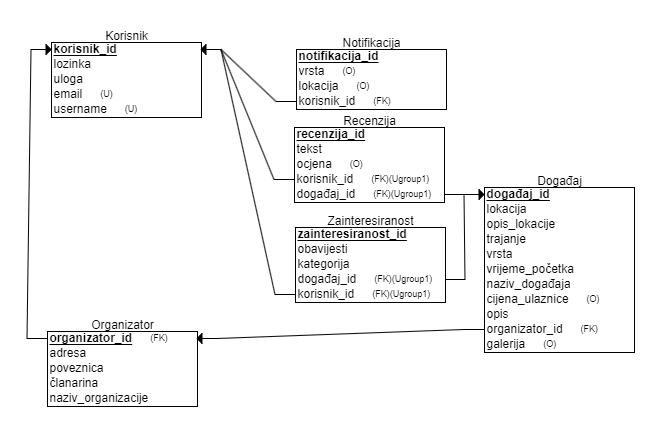
\includegraphics[scale=0.7]{slike/baza.PNG}
					\caption{Dijagram baze podataka}
				\end{figure}
			\eject
			
			
		\section{Dijagram razreda}
		
			\textit{Potrebno je priložiti dijagram razreda s pripadajućim opisom. Zbog preglednosti je moguće dijagram razlomiti na više njih, ali moraju biti grupirani prema sličnim razinama apstrakcije i srodnim funkcionalnostima.}\\
			
			\textbf{\textit{dio 1. revizije}}\\
			
			\textit{Prilikom prve predaje projekta, potrebno je priložiti potpuno razrađen dijagram razreda vezan uz \textbf{generičku funkcionalnost} sustava. Ostale funkcionalnosti trebaju biti idejno razrađene u dijagramu sa sljedećim komponentama: nazivi razreda, nazivi metoda i vrste pristupa metodama (npr. javni, zaštićeni), nazivi atributa razreda, veze i odnosi između razreda.}\\
			
			\textbf{\textit{dio 2. revizije}}\\			
			
			\textit{Prilikom druge predaje projekta dijagram razreda i opisi moraju odgovarati stvarnom stanju implementacije}
			
			
			
			\eject
		
		\section{Dijagram stanja}
			
			
			\textbf{\textit{dio 2. revizije}}\\
			
			\textit{Potrebno je priložiti dijagram stanja i opisati ga. Dovoljan je jedan dijagram stanja koji prikazuje \textbf{značajan dio funkcionalnosti} sustava. Na primjer, stanja korisničkog sučelja i tijek korištenja neke ključne funkcionalnosti jesu značajan dio sustava, a registracija i prijava nisu. }
			
			
			\eject 
		
		\section{Dijagram aktivnosti}
			
			\textbf{\textit{dio 2. revizije}}\\
			
			 \textit{Potrebno je priložiti dijagram aktivnosti s pripadajućim opisom. Dijagram aktivnosti treba prikazivati značajan dio sustava.}
			
			\eject
		\section{Dijagram komponenti}
		
			\textbf{\textit{dio 2. revizije}}\\
		
			 \textit{Potrebno je priložiti dijagram komponenti s pripadajućim opisom. Dijagram komponenti treba prikazivati strukturu cijele aplikacije.}